\section{Experiment}
% prof suggestion :: still under implementation. We are planning to do this & this. We are expecting result like this

Due to the nature of MARL and our game rules, we don't need any prior data collection. Reinforcement learning will collect data as each game is played. We have implemented a simulation of the game described in section~\ref{Game Description} along with the three different MARL AI implementations. The different MARL AI are pitted against each other over a series of games to measure how each AI learns based on the number of wins, and average score, calculated by equation~\ref{eqn:score}.

To meausre how each AI learns, we take a set window of games and evaluate the number of wins, average score, and average turns to win seperate from all other windows. For 10000 games, each window is of size 1000 games and will show the progress in learning every 1000 games. Scores are listed above wins in each graph as a difference between the two team's scores.
%High performance is indicated by higher win success rates with higher average scores and lower average turns to win.

 \begin{figure}[htb]

\begin{minipage}[b]{1.0\linewidth}
  \centering
  \centerline{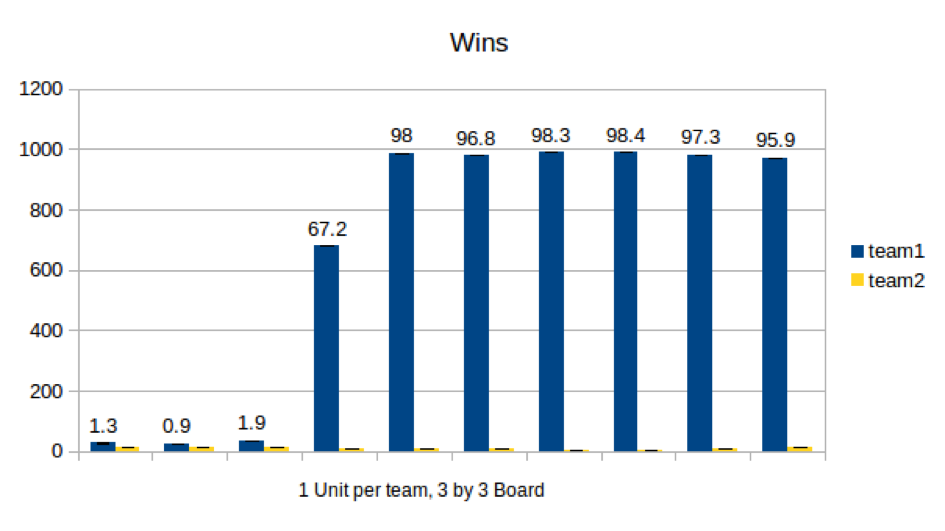
\includegraphics[width= 9 cm,height= 16 cm,keepaspectratio]{1v1}}
%  \vspace{2.0cm}
  
\end{minipage}
\caption{One unit in each team in a 3 by 3 board}
\label{fig:1v1}
%
\end{figure}

The first experiment sets both team sizes to 1 unit each with a board size of 3 by 3 and runs 10000 games. With only 1 unit per team, no information can be shared between units so each algorithm should perform the same in terms of learning. WIth a board size of 3 by 3, both units are able to reach each other and kill the enemy within a single turn. As a unit learns from game to game it should explore most, if not all, of the state-action space and eventually the action of killing an enemy will be discovered and reinforced positively. After enough runs, the team who takes the first turn should win every time since it will have positively reinforced the action of killing the enemy within a single turn. Looking at Figure~\ref{fig:1v1}, it is evident that one team was the clear overall winner. As you can see, during the first couple thousand games neither team was beating the other. Eventually, team 1 learned how to kill team 2. At this point, due to the bias nature of the game setup, team 1 fully learned how to win almost every game.
%Looking at Table~\ref{tab:SanityCheck}, it is evident that one team was the clear overall winner. It is also evident that on average the number of turns taken for either team to win is only a single turn, or close to it.



The second experiment sets both team sizes to $3$ on a board of size $5$ by $8$, and runs for $10000$ games. This is a larger board and both teams are bigger, giving each algorithm room to learn differently. With more than $1$ unit per team, sharing becomes a factor as well so here we expect to see Oracle outperform both Independent and Cooperative. We also expect to see Cooperative outperform Independent. Over 10000 games, we see in Figure-~\ref{fig:CvO} and Figure-~\ref{fig:IvO} that indeed oracle does win more often and with a higher score than the other two algorithms. Cooperative also outperforms Independent, but by an even slighter margin [Figure-~\ref{fig:IvC}]. As the win rate, and score are within small bounds when comparing one algorithm to another, we believe this leaves room for further improvement, discussed in section ~\ref{futurework}. The red curve in figure-\ref{fig:IvC}, figure-\ref{fig:CvO}, figure-\ref{fig:IvO} is reflecting the learning rate of the agents.
%Table~\ref{tab:TrueExperiment} that indeed oracle does win more often and with a higher score than the other two algorithms. Cooperative also outperforms Independent in score and turns taken to win, but by an even slighter margin. As the win rate, score, and turn average are within small bounds when comparing one algorithm to another, we believe this leaves room for further improvement, discussed in section ~\ref{futurework}

\begin{figure}[htb]

\begin{minipage}[b]{1.0\linewidth}
  \centering
  \centerline{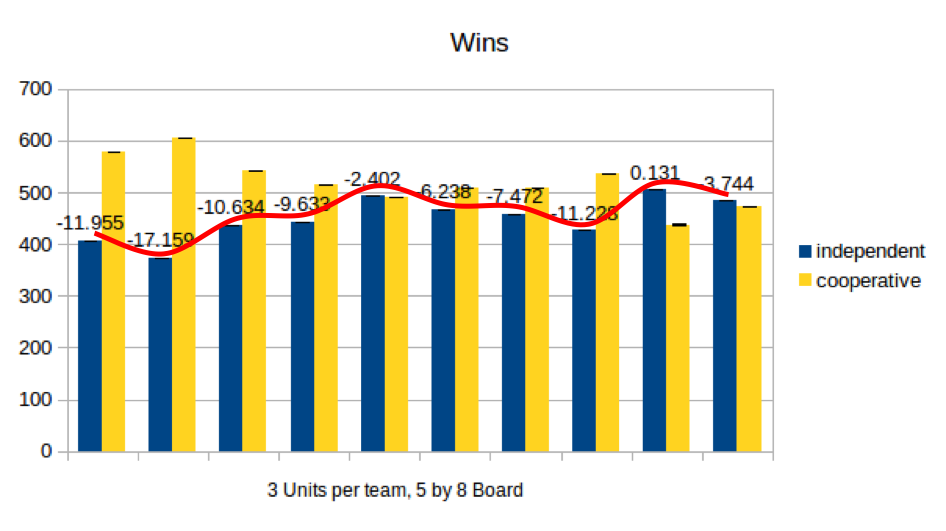
\includegraphics[width= 9 cm,height= 16 cm,keepaspectratio]{IvC}}
%  \vspace{2.0cm}
  \caption{Independent vs Cooperative teams with 3 units in each team in a 5 by 8 board}
\label{fig:IvC}
\end{minipage}
\end{figure}

\begin{figure}[htb]
\begin{minipage}[b]{1.0\linewidth}
  \centering
  \centerline{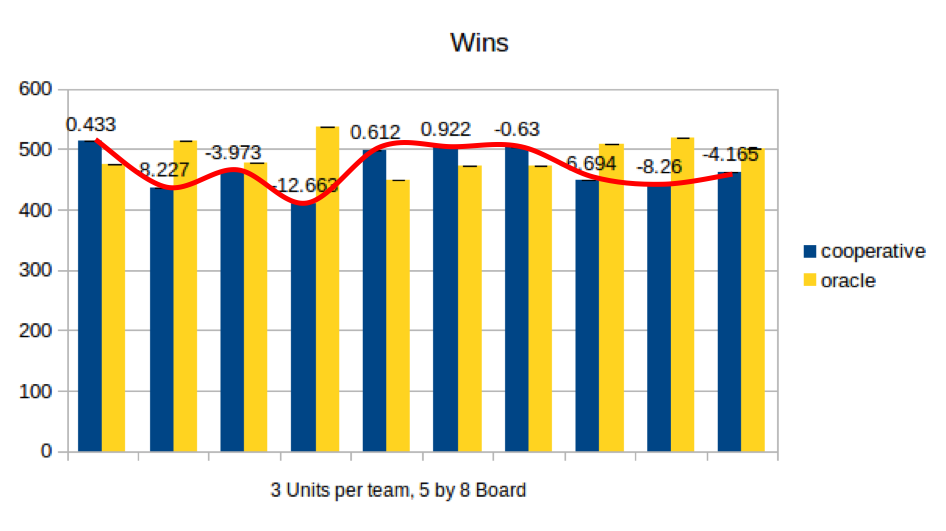
\includegraphics[width= 9 cm,height= 16 cm,keepaspectratio]{CvO}}
%  \vspace{2.0cm}
  \caption{Cooperative vs Oracle teams with 3 units in each team in a 5 by 8 board}
\label{fig:CvO}
\end{minipage}
\end{figure}

\begin{figure}[htb]
\begin{minipage}[b]{1.0\linewidth}
  \centering
  \centerline{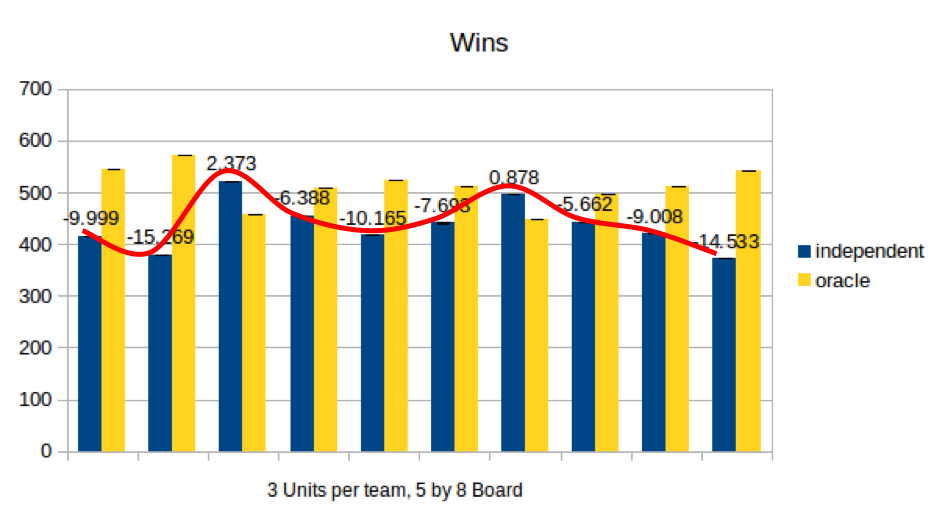
\includegraphics[width= 9 cm,height= 16 cm,keepaspectratio]{IvO}}
%  \vspace{2.0cm}
  \caption{Independent vs Oracle teams with 3 units in each team in a 5 by 8 board}
\label{fig:IvO}
\end{minipage}

%
\end{figure}


%that indeed Oracle does win more often and with a higher score against the other two algorithms. Cooperative also shows to outperform Independent in score and turns taken to win. The win rate, score, and turn average are with small bounds when comparing one algorithm to another and we believe this leaves room for further improvement, discussed in~\ref{futurework}.

%%%% basing on the number of games, show a table to compare the learning

\iffalse
\begin{table}[htbp] \hspace{-1cm}
\centering
\begin{tabular}{c|c|c|c}
 & Wins & Score & Turns  \\ \hline
Oracle & 0.82 (0.003) & 80.14 (0.33) & 2.26 (0.005)\\
vs. Independent & 0.17 (0.003) & 15.42 (0.33) & 1.96 (0.003)\\ \hline
Independent & 0.02 (0.001) & 1.44 (0.13) & 1 (0)\\
vs. Cooperative & 0.97 (0.001) & 96.55 (0.13) & 1 (0)\\ \hline
Cooperative & 0.02 (0.001) & 1.25 (0.13) & 1 (0) \\
vs. Oracle & 0.97 (0.001) & 96.74 (0.13) & 1 (0)
\end{tabular}
\caption{Team Size: 1, Board Size: 3 x 3, 50000 games. Results are read as: value (+/- confidence in value)}
\label{tab:SanityCheck}
\end{table}



\begin{table}[htbp] \hspace{-1cm}
\centering
\begin{tabular}{c|c|c|c}
 & Wins & Score & Turns  \\ \hline
Oracle & 0.54 (0.009) & 65.39 (0.58) & 9.75 (0.16)\\
vs. Independent & 0.45 (0.009) & 58.23 (0.61) & 10.94 (0.19)\\ \hline
Independent & 0.5 (0.009) & 62.41 (0.59) & 10.61 (0.15)\\
vs. Cooperative & 0.5 (0.009) & 65.56 (0.55) & 9.67 (0.15)\\ \hline
Cooperative & 0.48 (0.009) & 63.33 (0.57) & 10.13 (0.15) \\
vs. Oracle & 0.51 (0.009) & 62.55 (0.59) & 11.17 (0.16)
\end{tabular}
\caption{Team Size: 3, Board Size: 6 x 9, 10000 games. Results are read as: value (+/- confidence in value)}
\label{tab:TrueExperiment}
\end{table}

\vspace{-.5 cm}
\fi